\chapter*{Conclusion et perspectives}
\markboth{Conclusion et perspectives}{Conclusion et perspectives}
\addcontentsline{toc}{chapter}{Conclusion et perspectives}
\setcounter{figure}{0}
\renewcommand{\thefigure}{Concl.\arabic{figure}}

Les différents travaux réalisés durant ma thèse ne sont que les premières étapes dans le développement d'une véritable spintronique à l'échelle de la molécule unique. Ils ont cependant révélé de nombreux aspects très prometteur quant à l'utilisation de l'interaction entre le transport électronique et le magnétisme moléculaire. Grâce à la réalisation d'un transistor à molécule unique basé sur l'utilisation d'un aimant moléculaire (Fig.\ref{Conclusion1}.\textbf{a}), la faisabilité d'une spintronique moléculaire a été démontrée. Elle permet notammant de sonder, à l'échelle d'un moment magnétique unique, le magnétisme moléculaire.


\begin{figure}
\centering 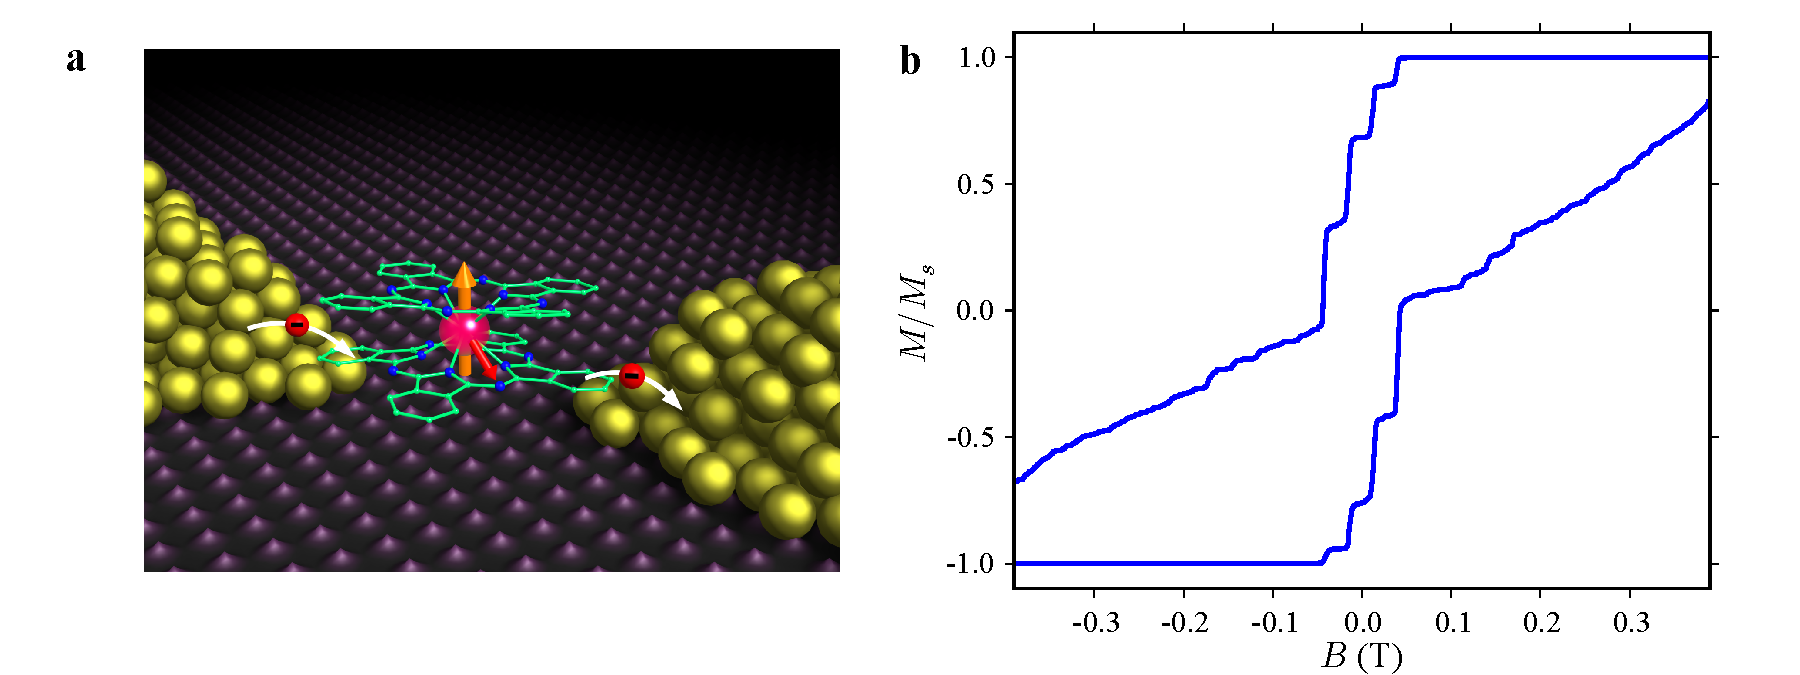
\includegraphics[scale=0.45]{Conclusion/Conclusion1/Conclusion1.pdf} 
\caption{\textbf{a} : vue d'artiste de notre transistor moléculaire. \textbf{b} : reconstitution du cycle d'hystéresis de la molécule TbPc$_2$ pour un champ transverse de $750\,mT$.}
\label{Conclusion1}
\end{figure}


Nous avons tout d'abord montré que la conductance de notre transistor était dépendante de l'orientation du moment magnétique d'une seule molécule. Cette propriété nous a permis d'observer le retournement de l'aimantation par effet tunnel à l'échelle d'un moment unique. Cette capacité de mesure fait également, de notre technique, un détecteur d'une très grande sensibilité qui pourrait être utilisé, dans le cadre du magnétisme moléculaire, pour l'investigation des propriétés quantiques des aimants moléculaires. Afin de contribuer à cette étude, nous avons notamment développé une méthode permettant de reconstituer le cycle d'aimantation à l'échelle d'une molécule unique~(Fig.\ref{Conclusion1}.\textbf{b}). Cette mesure montre clairement les différences qu'il existe entre un cycle obtenu à partir d'une assemblée et celui correspondant à un aimant moléculaire~(cf Chap.3).


En outre, nous avons présenté une nouvelle technique, basée sur le phénomène de QTM, permettant de mesurer, de manière non destructive, l'état d'un spin nucléaire unique. Cette possibilité porte la sensibilité de notre technique à quelques millièmes de $\mu_B$. Nous avons ainsi pu étudier la dynamique d'un spin nucléaire et mettre en évidence le long temps de vie de l'état de spin, de l'ordre de 10 secondes. De plus, nous avons montré que la température du spin nucléaire était proche de la température électronique de notre réfrigérateur à dilution~(environ 80$\,mK$), témoignant d'une bonne thermalisation de ce dernier malgré le courant traversant le système. Ces différents résultats ouvrent donc la voie expérimentale à la proposition théorique de Kane~\cite{Kane1998} relatant de l'utilisation du spin nucléaire comme base d'une électronique quantique.


Cependant, certains aspects des mesures que j'ai présentées demeurent inexpliqués pour l'instant. En effet, si le rôle de l’environnement électrostatique, et donc le régime de transport, sur le magnétisme de notre aimant moléculaire est indiscutable, le ou les mécanismes régissant cette dépendance ne sont pas encore identifiés. Il conduisent pourtant à une modification de la vitesse de relaxation comme nous l'avons détaillé dans le Chap.3. De plus, le cycle d’hystérésis obtenu à partir de mesures faites en régime Kondo~(cf Fig.\ref{TransIndConcl}.\textbf{b}) semble montrer qu'il est possible de supprimer les transitions autres que QTM.  Reste également à expliquer la présence de transitions induites que l'on observe à fort champ magnétique~($\geq 100\,mT$) dans les mesures d’hystérésis~(cf Chap.3). Une première étude de leurs positions en fonction du champ parallèle et du champ transverse (cf Fig.\ref{TransIndConcl}.\textbf{a}) nous permet de penser que ces dernières sont dues à l'interaction entre la molécule et un second système magnétique. Mais la nature de ce système et de l'interaction qui le couple à l'aimant moléculaire restent encore à déterminer. Il apparaît primordial de démontrer si ces différents phénomènes ne sont que les manifestations d'un seul et même mécanisme. De manière plus générale, une compréhension accrue des phénomènes de couplage entre le magnétisme moléculaire et son environnement nous parait indispensable.

\begin{figure}[h!]
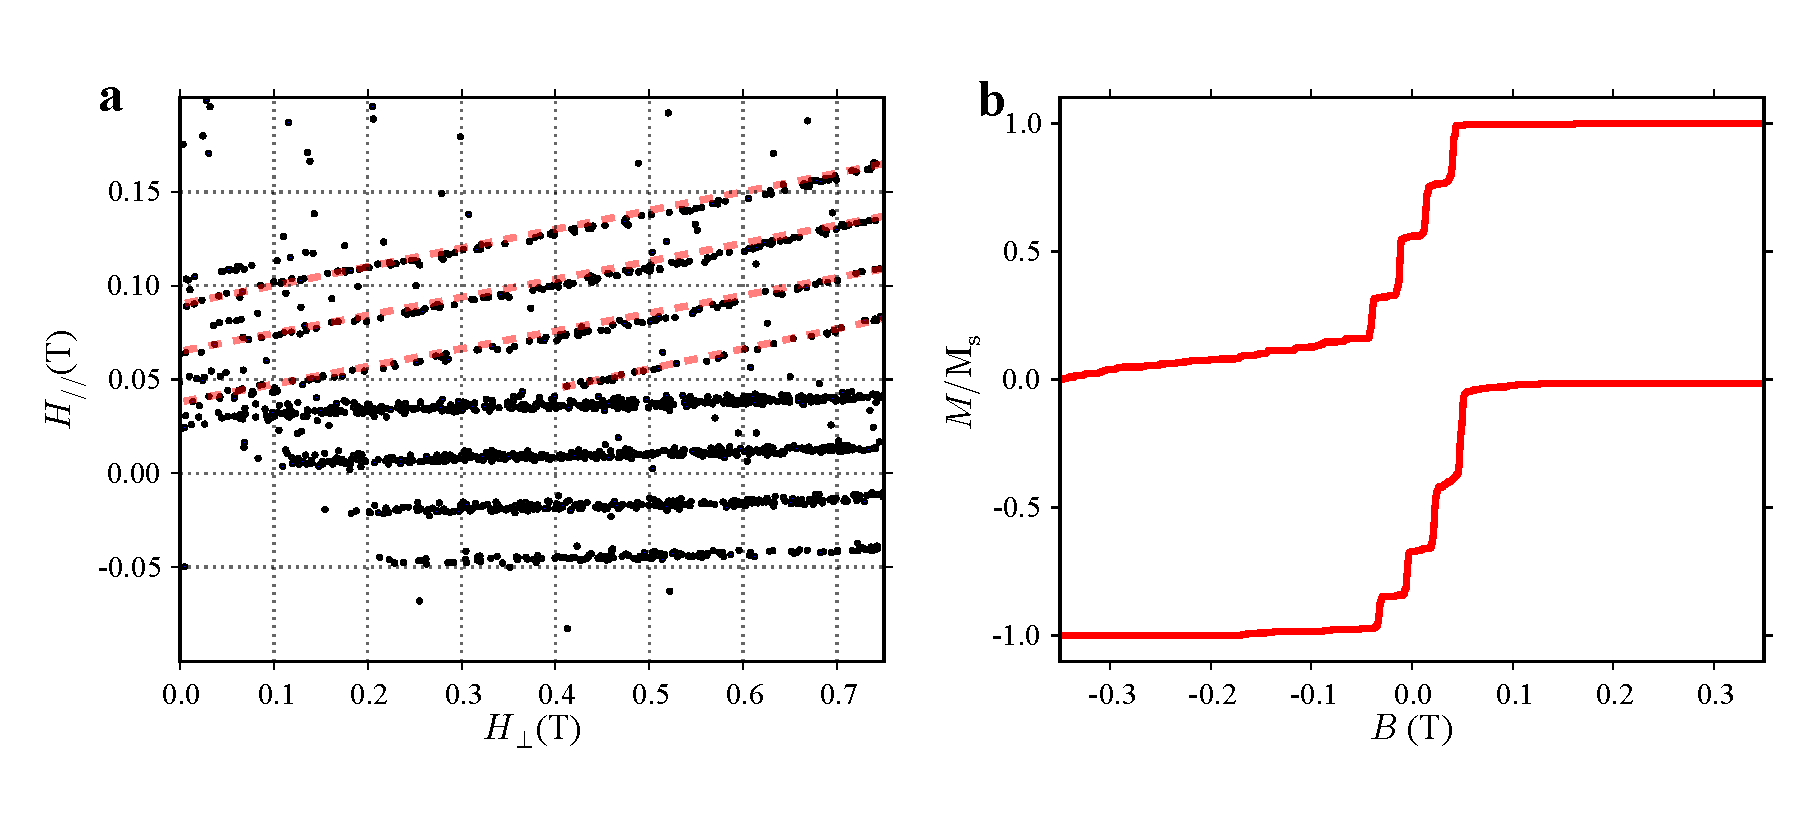
\includegraphics[scale=0.45]{Conclusion/TranInd/TransInd.pdf} 
\caption{\textbf{a} : étude de la position des transitions induites en fonction du champ transverse et du champ parallèle. Chaque point marque un retournement de l'aimantation. Les transitions surlignées en rose correspondent à des renversements de l'aimantation induits par le couplage de l'aimant moléculaire avec un second système magnétique. \textbf{b} : reconstruction du cycle d'hystérésis obtenu en régime Kondo. Seules les transitions correspondantes au phénomène de QTM sont visible.}
\label{TransIndConcl}
\end{figure}


De plus, notre technique de réalisation de transistor à molécule unique mériterait d’être perfectionnée en exploitant les possibilités offertes par l’approche ``\textit{Bottom-Up}". C'est une voie que nous avons commencée à développer, dans le cadre de la thèse de Sébastien Liatard~\cite{Liatard2012}, en collaboration avec le Département de Chimie Moléculaire de l’Université Joseph Fourier. L’un des objectifs de ce travail de thèse consistait en l’utilisation de nanoparticules d'or pour la connexion d’une molécule unique. En effet, comme l'on déjà réalisé l'équipe de T. Bjørnholm~\cite{Jain2009} avec une molécule de HS-PEG-SH (PEG = polyéthylène glycol), il est possible d'attacher une molécule possédant deux groupements thiols à deux nanoparticules d'or de très petite taille (3-5\,nm), puis de faire croître ces particules sous forme de bâtonnets d'une longueur atteignant 500\,nm, et ne dépassant pas 30\,nm de largeur. Ces bâtonnets sont alors facilement repérables par microscopie, et peuvent être connectés à des électrodes afin d'être inclus dans un circuit électrique. La synthèse de ces bâtonnets a été développée par Murphy et al.~\cite{Murphy2006} et permet de produire des nano-objets unidimensionnels de taille contrôlée, grâce à l'utilisation dans le milieu de croissance d'un surfactant en forte concentration. 

\begin{figure}[h!]
\parbox{7cm}{
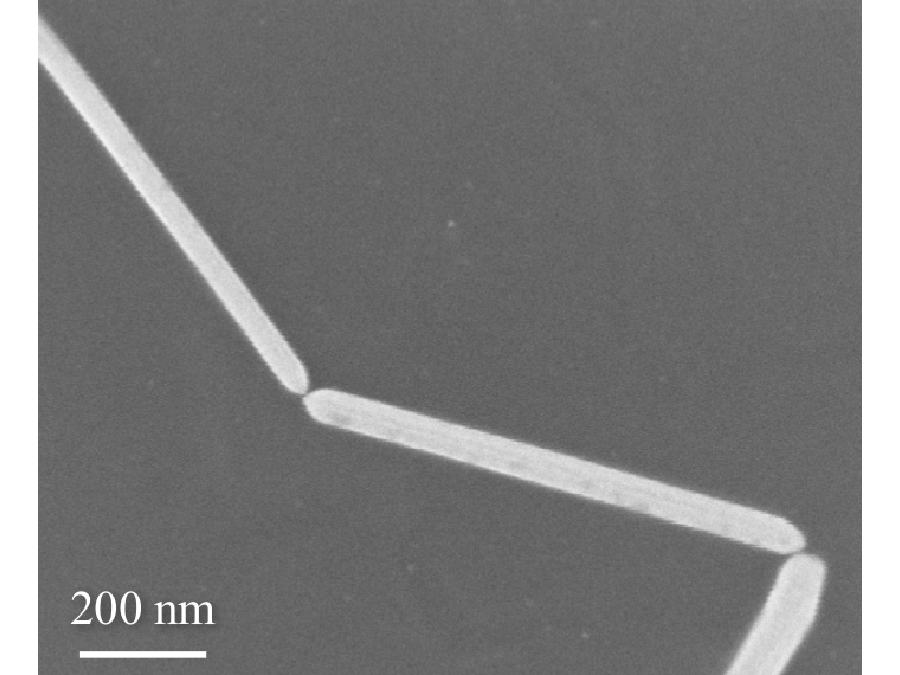
\includegraphics[scale=0.45]{Conclusion/BottomUp/BottomUp.pdf} 
}
\parbox{6.5cm}{\caption{Configuration idéale, bien que très peu reproductible pour l'instant,
de bâtonnets d'or joints bout-à-bout par une ou quelques molécules~(extrait de~\cite{Liatard2012}).}
\label{BottomUpConclu}
}
\end{figure}

Nous avons donc commencé à travailler sur ces bâtonnets d'or, et essayé notamment de reproduire les expériences de Murphy \textit{et al.}. La Fig.\ref{BottomUpConclu} montre un cas particulier de bâtonnets liés bout-à-bout. Idéalement, c'est le type d'assemblage que nous cherchons à obtenir, avec une molécule unique dans l'interstice entre les bâtonnets. Cependant, si la production de bâtonnets ne présente pas de difficultés majeures, leur purification est plus ardue, la synthèse produisant en effet d'autres particules d'or de différentes formes. La séparation, faite par centrifugation principalement, de ces différents types de particules, est difficile. Malgré les difficultés rencontrées, il nous paraît nécessaire de poursuivre dans cette voie afin d’obtenir des dispositifs en plus grand nombre et de manière reproductible. On pourra ainsi imaginer l’utilisation des techniques ``\textit{Bottom-Up}" pour la réalisation de mémoires entièrement constituées de jonctions moléculaires, permettant ainsi d’atteindre des densités de stockage exceptionnelles.

\begin{figure}[h!]
\parbox{7cm}{
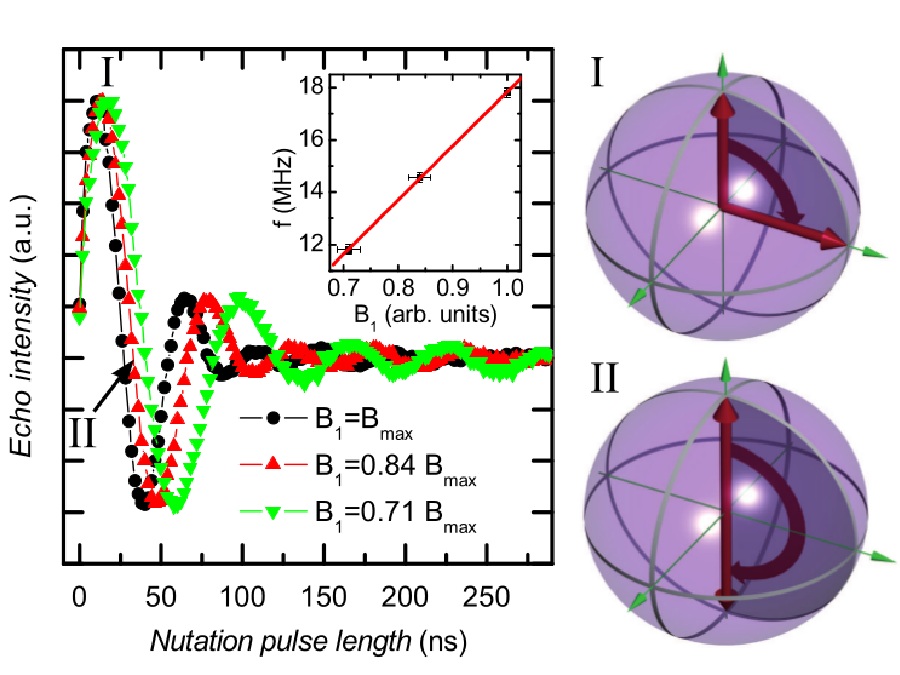
\includegraphics[scale=0.45]{Conclusion/OscilFe4/OscilFe4.pdf} 
}
\parbox{6.5cm}{\caption{(lignes de couleur) Oscillations de Rabi obtenues en enregistrant l'intensité de l'écho en fonction de la durée de pulsation sur du Fe$_4$ à très basse température et pour différents champs magnétiques. Pour deux positions dans le cycle de Rabi, la position correspondante est présentée dans la partie droite~(extrait de~\cite{Schlegel2008}).}
\label{OscilFe4}
}
\end{figure}

L'utilisation des aimants moléculaires comme brique élémentaire de l'information quantique a été proposée dans de nombreux travaux. Elle a également été illustrée par la mesure d'oscillations de Rabi sur des molécules de Fe$_{4}$(cf~\cite{Schlegel2008} et Fig.\ref{OscilFe4}). Mais il s'agissait, dans la plupart de ces travaux, d'utiliser le moment magnétique électronique comme support de l'information. Nos travaux montrent que la manipulation et la lecture des états du spin nucléaire constituent une piste prometteuse vers la réalisation d'un qbit à base d'aimant moléculaire. Si nous avons démontré comment réaliser l’étape de lecture, reste encore à mettre en œuvre l’étape de manipulation. 

\begin{figure}[h!]
\parbox{7cm}{
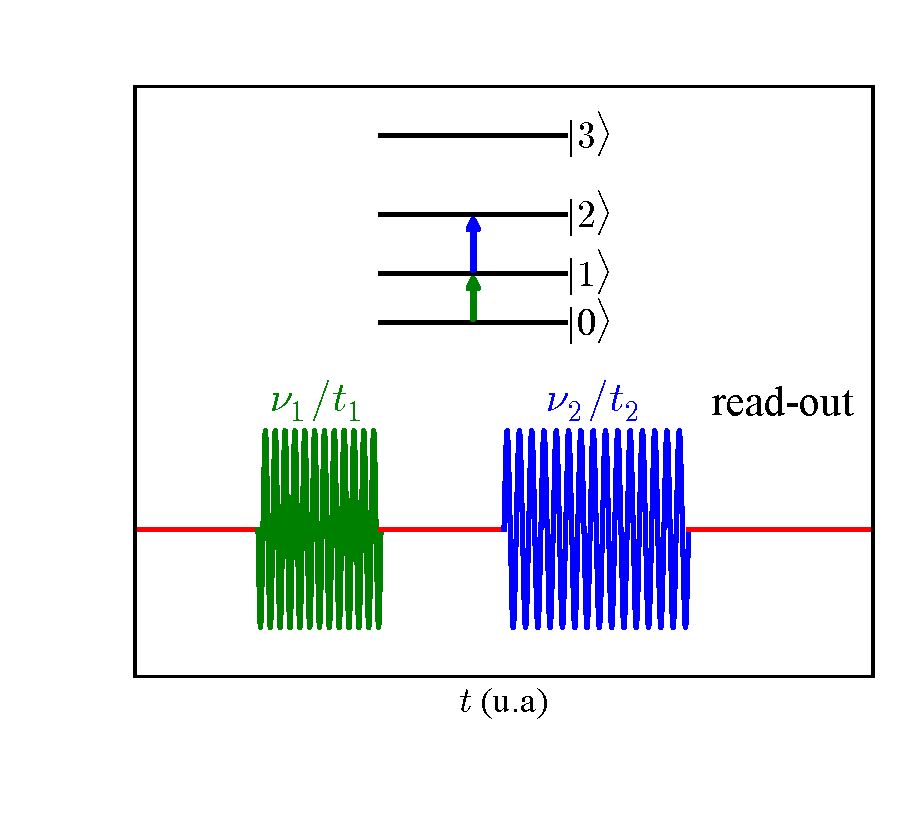
\includegraphics[scale=0.45]{Conclusion/spin_nuc_man/spin_nuc_man.pdf} 
}
\parbox{6.5cm}{\caption{Schéma de la technique de pompe-sonde. Une première fréquence $\nu_1$ initialise l'état de $|0\rangle$ à l'état $|1\rangle$. Puis un second pulse fait passer le système de l'état $|1\rangle$ à l'état $|2\rangle$. On effectue ensuite la lecture de l'état par la méthode présentée au Chap.3.}
\label{spin_nuc_man}
}
\end{figure}

On pourrait pour cela profiter de l'espacement inégal des énergies des différents états de spin, pour implémenter un schéma de pompe/sonde comme présenté dans la Fig.3.1.d. Une première étape consistant en un pulse d'une fréquence $\nu_1$ initialiserait le spin nucléaire de l’état $|0\rangle$ à l'etat $|1\rangle$. Un temps variable séparerait cette étape d'un second pulse de fréquence $\nu_2$ permettant la transition de l’état $|1\rangle$ à l’état $|2\rangle$. La lecture se ferait ensuite par la procédure que l'on a présentée dans le Chap.3. On pourrait ainsi mettre en évidence des oscillations de Rabbi par des mesures en transport, accédant au $T_2$ du spin nucléaire, et réaliser le premier qbit à base d'aimant moléculaire.

Du fait de la répartition anharmonique des niveaux d’énergies du spin nucléaire, une procédure plus complexe pourrait également être développée mettant en jeux un nombre plus élevé de pulses radio-fréquences (RF) dont la polarisation serait contrôlée. Une telle procédure permettrait d’implémenter l'algorithme de Grover, comme cela a été détaillé par Loss et al. dans~\cite{Leuenberger2003}.

%\begin{figure}
%\centering 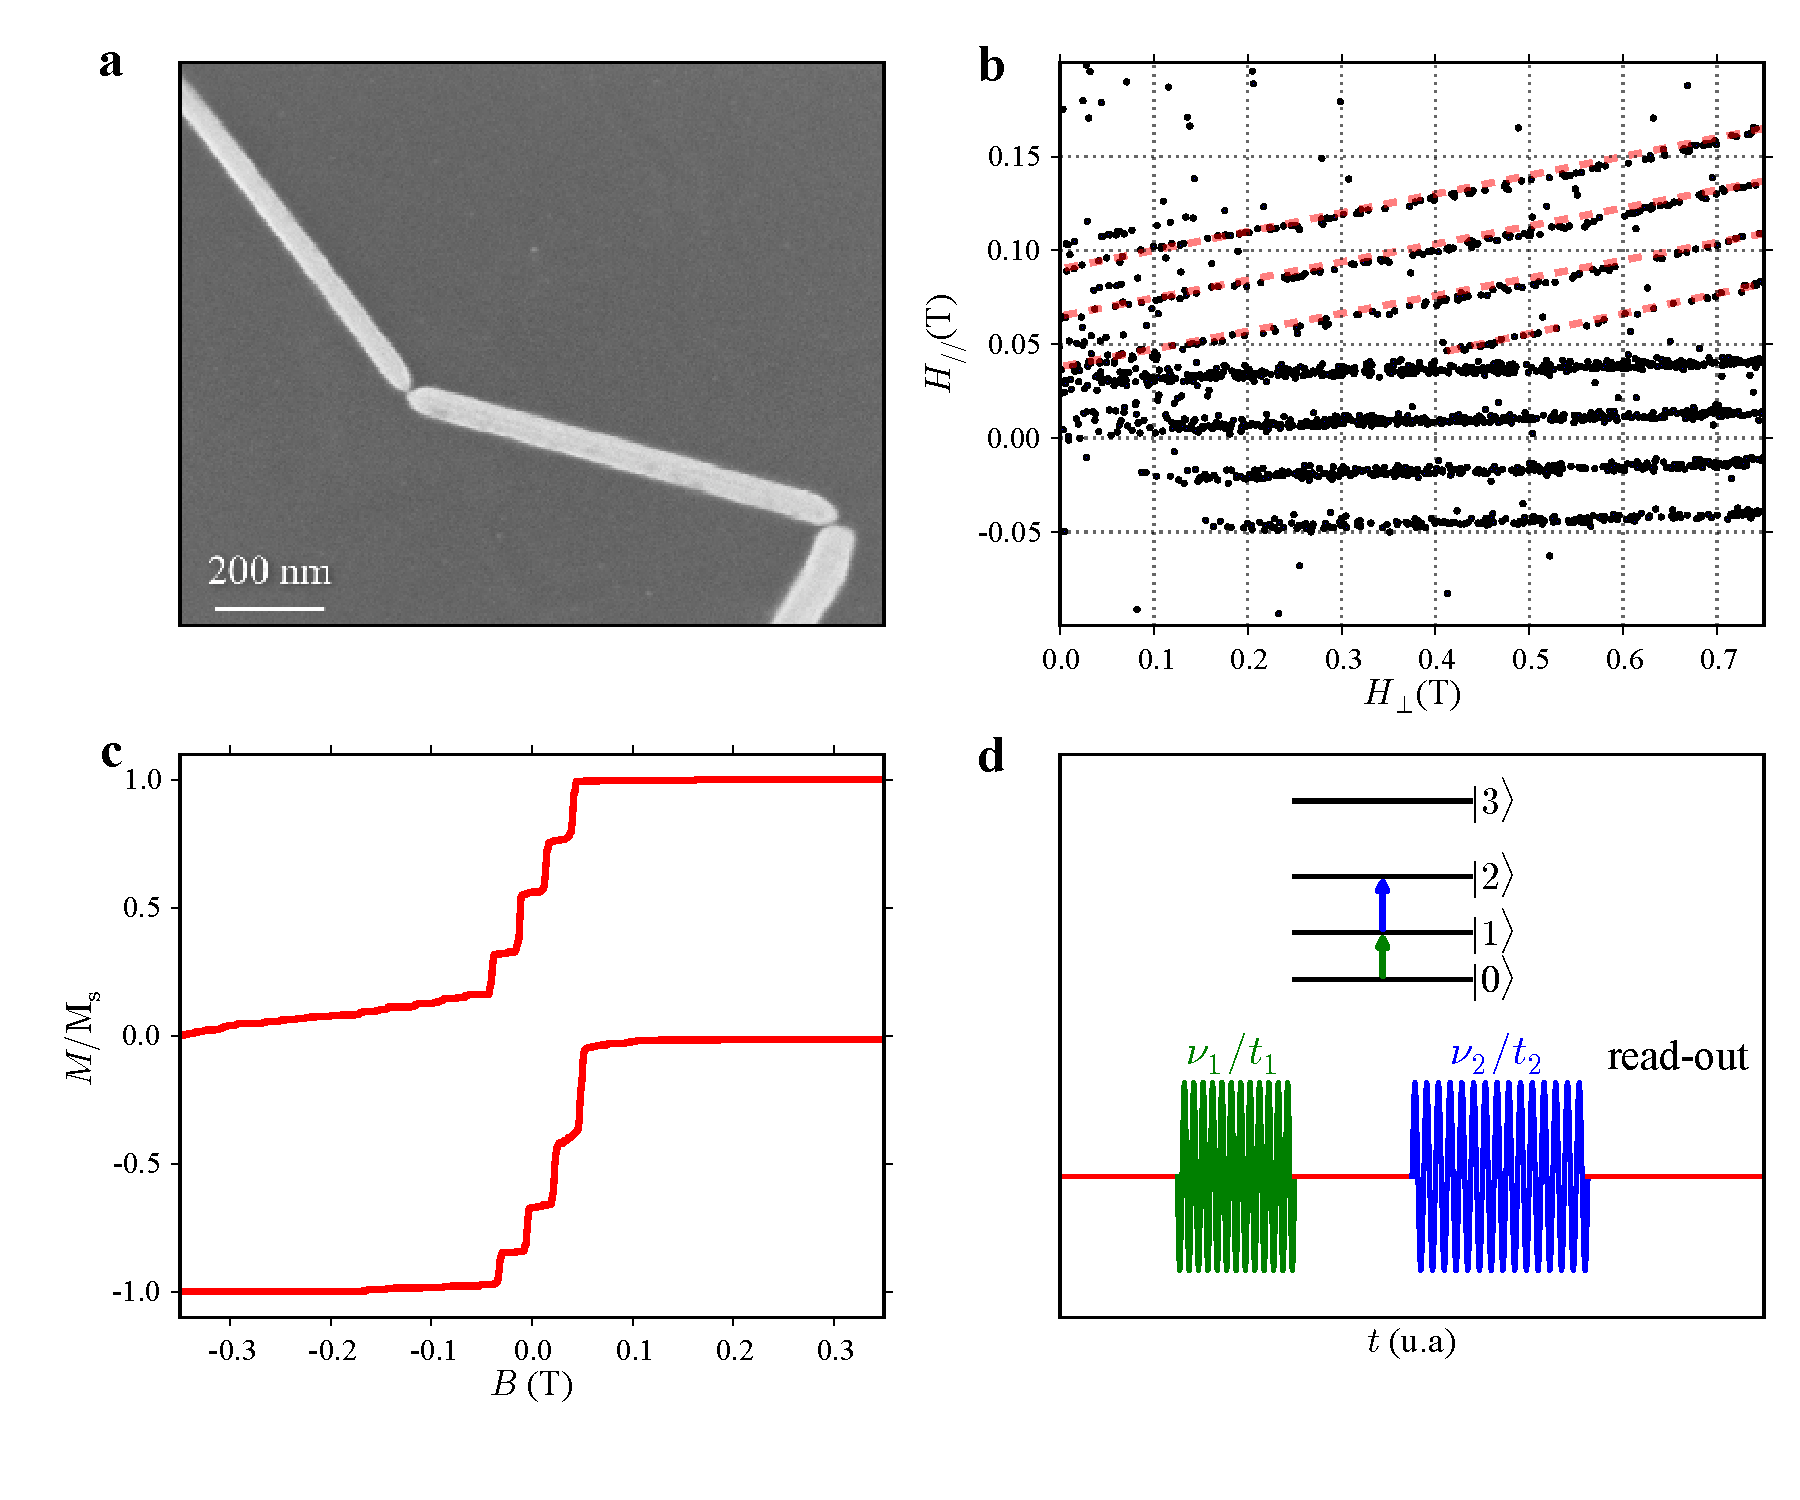
\includegraphics[scale=0.45]{Conclusion/Perspectives/Perspectives.pdf} 
%\caption{\textbf{a} : deux bâtonnets d'or obtenus à partir de la croissance de deux billes d'or reliées entre-elles par des molécules~(extrait de [thèse de Sebastien]). \textbf{b} : étude de la position des transitions induite en fonction du champ parallèle et du champ transverse. Chaque point marque un retournement de l'aimantation. Les transitions surligné en rose corresponde à des renversements induits par le couplage de l'aimant moléculaire avec un seconde système magnétique. \textbf{c} : reconstruction du cycle d'hystérésis obtenu en régime Kondo. Seules les transitions correspondantes au phénomène de QTM sont visible. \textbf{d} : schéma de la technique de pompe-sonde. Une première fréquence $\nu_1$ initialise l'état de $|0\rangle$ à l'état $|1\rangle$. Puis un second pulse fait passer le système de l'état $|1\rangle$ à m'état $|2\rangle$. On effectue ensuite la lecture de l'état par la méthode présentée au Chap.3.}
%\label{Perspectives}
%\end{figure}

